 \documentclass[conference]{IEEEtran}
\IEEEoverridecommandlockouts
%\usepackage{hyphenat}
\usepackage[ruled,vlined]{algorithm2e}
\usepackage{amsmath}
\usepackage{xspace}
\usepackage[binary-units=true]{siunitx}
\usepackage{ulem}
%\usepackage{censor}
\usepackage[table]{xcolor}
\usepackage{graphicx}
\usepackage{hyperref}
\usepackage{tabularx}

\usepackage{subcaption}
\usepackage{booktabs}
\usepackage{multirow}
\usepackage{listings}
\usepackage{dingbat}

\hypersetup{
    colorlinks=true,
    linkcolor=black,
    citecolor=blue,
    filecolor=black,
    urlcolor=blue}

\def\BibTeX{{\rm B\kern-.05em{\sc i\kern-.025em b}\kern-.08em
    T\kern-.1667em\lower.7ex\hbox{E}\kern-.125emX}}

\begin{document}

\newcommand{\fslspm}{FSL-SPM\xspace}
\newcommand{\fslafni}{FSL-AFNI\xspace}
\newcommand{\afnispm}{AFNI-SPM\xspace}
\newcommand{\tristan}[1]{\color{orange}\textbf{From Tristan:} #1\color{black}\xspace}
\newcommand{\ali}[2]{\color{green}\textbf{Ali:} #1\color{black}\xspace}



\title{Comparing tool variability and numerical variability in fMRI analyses}

\author{Ali Salari$^1$, Other Authors$^1$, Tristan Glatard$^1$ \\
$^1$ Department of Computer-Science and Software Engineering, Concordia University, Montreal, Canada}

\maketitle
\begin{abstract}

Numerical and software variability broadly affect structural, diffusion, and functional MRI analyses. Numerical
variability originates in software updates or code
parallelization, whereas software variability reflects discrepancies between
models implemented in different analysis software packages. While numerical
and software variability were both shown to impact analysis outcomes, the
extent to which these sources of variability compare for a given
analysis remains understudied. This work presents a comparison of
numerical and software variability for group-level functional MRI analysis
\tristan{did we give up on individual analyses?}.
We reproduced a previous comparison between functional MRI analysis
software packages FSL, AFNI, and SPM, which we extended to measure
numerical variability through Monte-Carlo arithmetic.
We find that between-tool variability is an order of magnitude higher than numerical variability.
\tristan{summarize conclusions}

\end{abstract}

\begin{IEEEkeywords}
  Numerical Instability, Reproducibility, Monte-Carlo arithmetic, Neuroimaging
\end{IEEEkeywords}


\section{Introduction}

% Data analysis workflows in many scientific domains have become increasingly complex and flexible.
Recent studies highlighted the instability of the neuroimaging pipelines depending on the computing platform,
software package, and even tool versions. Changes in the computational
environment such as compilers, libraries, operating systems may introduce small numerical errors and create
significantly different results in unstable pipelines~\cite{Glatard2015,Gronenschild2012,salari2020spot}.
Moreover, the impact of methodological changes on fMRI analyses has been investigated extensively~\cite{bowring2019exploring,botvinik2020variability,bhagwat2021understanding,carp2012plurality}.
For instance, in related works, it has been shown that running the same fMRI experiments by different teams can substantially affect
scientific conclusions~\cite{botvinik2020variability,carp2012plurality};
replication of fMRI experiments using the three most well-known software packages can influence the final determining areas of
brain activations~\cite{bowring2019exploring}; %bowring2021isolating.
also, the choice of preprocessing pipelines on neuroimaging cortical surface analyses is compound with instabilities~\cite{bhagwat2021understanding}.
% In the presence of such instabilities, it is often hard to trust the data processing results. % validity of the computational results.

In such a heterogeneous environment, numerical instability is an essential issue for reproducibility.
Numerical instability is a characteristic of pipelines that results from the influence of the floating-point arithmetics
and iterative convergence of numerical errors~\cite{freitas2002issue}.
Stochastic arithmetic approaches such as Monte-Carlo arithmetic (MCA)~\cite{Parker1997-qq} have been used to study the impact of numerical errors
originating in floating-point computations in mathematical libraries.
In~\cite{salari2021accurate}, we quantified the numerical stability of the HCP preprocessing pipeline~\cite{glasser2013} based on the MCA method
by creating a Fuzzy environment, so that instrument mathematical functions are implemented in mathematical system libraries.
As a result of numerical perturbations, we discovered a very low numerical precision in the result images comparable to the operating system variability.
In a related study~\cite{kiar2020numerical}, the instability of results was explored by instrumenting a connectome estimation pipeline with the MCA technique.
These works demonstrate the necessity of numerical uncertainty quantification for understanding related issues that hamper the computational reproducibility of analyses.

In this work, we reproduce an fMRI analysis in~\cite{bowring2019exploring} with different neuroimaging software packages in the presence of the Fuzzy environment,
and then quantify the variability across tools and the numerical variability in results.
We call the cross-software variation and numerical variation, between tool (BT) and within tool (WT) variability, respectively.
In fact, the WT variability shows results across software packages in the Fuzzy environment.
The primary objective of this study is to answer these two questions: 1) how the fMRI analyses across tools are numerically stable?
2) how the numerical variability is in comparison with the tool variability?
This comparative study reveals the importance of numerical variability and motivates research studies to evaluate the numerical uncertainty of the pipelines.

% We start to reproduce an analysis from Bowring, this can be as a practice for reproducibility manner in the community.
% In particular, we investigate the effect of 1) between software 2) within software (numerical)
% We present a comparative assessment of group-level analysis of an fMRI pipeline.


\section{Materials and Methods}

\subsection{Fuzzy libmath environment}

To simulate uncertainty close to the level of machine error,
the maximum relative error due to rounding in floating-point arithmetic,
we used the method introduced in~\cite{salari2021accurate}
called Fuzzy libmath (FL). FL uses MCA to
% create an instrumented version of the functions embedded in the mathematical library in GNU operating systems (libmath) in which
introduce a controlled amount of noise in the floating-point operations embedded
in the mathematical library in GNU operating systems (libmath)
through the following perturbation model:
\begin{equation} \label{eq:mca_inexact}
  inexact(x) = x + 2^{e_x-t}\xi
\end{equation}
where $e_x$ is the exponent in the floating-point representation of $x$,
$t$ is the virtual precision, the number of bits in mantissa that will not be perturbed,
and $\xi$ is a random uniform variable of $(-\frac{1}{2}, \frac{1}{2})$.
The perturbation is applied in a given number of least-significant bits,
which models floating-point rounding and catastrophic cancellation errors.
This is automated using Verificarlo tool~\cite{denis2015verificarlo} that implements MCA at compilation time.

The instrumented functions are loaded in the pipeline using LD\_PRELOAD, a Linux environment variable
to force load a shared library into an executable. This allows functions defined in FL to transparently
overload the original ones without the need to modify or recompile the analysis pipeline.

To avoid some pitfalls in deterministic arithmetics like producing results out of the function definition,
FL instruments the functions by wrapping them so that only the original functions' output
is perturbed instead of input or their implementation.
Listing~\ref{algo:wrapper} shows an example of this wrapping for the log function in both single and double precisions.
In this script, the original functions are called by \texttt{dlsym},
a function that returns the memory address of a symbol using the handle of \texttt{RTLD\_NEXT}.
This allows one to provide a wrapper around a function in another shared library.
Also, the MCA instrumentation is activated by adding a floating-point zero to the output of the original function
so that the result of this summation is perturbed and returned.


% \lstdefinestyle{customc}{
%   belowcaptionskip=1\baselineskip,
%   breaklines=true,
%   frame=L,
%   xleftmargin=\parindent,
%   language=C,
%   showstringspaces=false,
%   basicstyle=\footnotesize\ttfamily,
%   keywordstyle=\bfseries\color{green!40!black},
%   commentstyle=\itshape\color{purple!40!black},
%   identifierstyle=\color{blue},
%   stringstyle=\color{orange},
% }

\lstdefinestyle{customasm}{
  belowcaptionskip=1\baselineskip,
  frame=L,
  xleftmargin=\parindent,
  language=[x86masm]Assembler,
  basicstyle=\footnotesize\ttfamily,
  commentstyle=\itshape\color{purple!40!black},
}
\lstinputlisting[caption=Sample wrapper script, label=algo:wrapper, style=customasm]{wrapper.c}
%\lstinputlisting[caption=Scheduler, style=customc]{../wrapper2.c}

FL allows measuring the effect of numerical variability by running a program multiple times
with the feature of controlling the magnitude of the perturbations as perceived by the application.
FL enables us to assess the software packages that are dynamically linked to the mathematical library.
So, it is important to trace the tool dependencies of the pipelines to understand the different libraries
involved during the pipeline executions.


\subsection{fMRI analysis \& Dataset}

We replicated the fMRI analysis described as study `ds000001' in~\cite{bowring2019exploring}, relying on
the data publicly available in OpenNeuro at \url{https://openneuro.org/datasets/ds000001}
and using the three main software packages for fMRI data processing, namely
FMRIB Software Library (FSL)~\cite{jenkinson2012fsl}, Analysis of Functional NeuroImages (AFNI)~\cite{cox1996afni},
and Statistical Parametric Mapping(SPM)~\cite{penny2011statistical}.
We selected this analysis because the methods and datasets were explicitly
written to be accessible and reproducible. This enabled us to reanalyze fMRI experiments using the FL framework and
compare WT and BT variabilities.

In the selected study, 16 healthy adult subjects participated in the balloon analog risk task to measure
risk-taking behavior over three scanning sessions.
This study included preprocessing, first-level, and second-level analyses that were implemented with all three software.
Table~\ref{table:pipeline-steps} shows the steps that were taken in the procedure of analyses for each tool in the original study.
In the original study, a number of preprocessing steps widely accepted within the community, such as motion correction,
segmentation, brain extraction, and registration, were applied in all analyses to ensure that results from each software
package could be compared objectively.
A full description of the pipelines implemented within three packages is presented in~\cite{bowring2019exploring,schonberg2012decreasing}.


%%%%%%%%%% Summary of statstics %%%%%%%%
\setlength{\tabcolsep}{4pt}
\begin{table}[h]
    \centering
    \begin{tabular}{|c|l|c|c|c|}
        \hline
%        \multirow{2}{*}{} & \multicolumn{1}{c}{Thresholded}& & \multicolumn{1}{c}{Unthresholded}& \\
        \multicolumn{2}{|c|}{} & FSL & AFNI & SPM \\
        \hline
        {Preprocessing} & {Motion Correction}                          & \checkmark    & \checkmark     & \checkmark  \\
        {} & {Segmentation}                               &    &      & \checkmark  \\
        {} & {Brain Extraction (Anatomical)}              & \checkmark     & \checkmark    & \checkmark  \\
        {} & {Brain Extraction (Functional)}              &   & \checkmark     &  \\
        {} & {Intra-subject Coregistration}               & \checkmark    & \checkmark     & \checkmark \\
        {} & {Inter-subject Registration}                 & \checkmark    & \checkmark     & \checkmark \\
        {} & {Analysis Voxel Size}                        & \checkmark    & \checkmark     & \checkmark \\
        {} & {Smoothing}                                  & \checkmark    & \checkmark     & \checkmark  \\
        \hline
        {First-level} & {Model Specification}                          & \checkmark    & \checkmark     & \checkmark  \\
        {} & {Inclusion of 6 Motion Parameters}                               & \checkmark   &  \checkmark    & \checkmark  \\
        {} & {Model Estimation}                           & &     & \checkmark  \\
        {} & {Contrasts}                                   &  \checkmark & \checkmark     & \checkmark \\
        \hline
        {Second-level} & {Model Specification}                          & \checkmark    & \checkmark     & \checkmark  \\
        {} & {Model Estimation}                           &      &    & \checkmark  \\
        {} & {Contrasts}                                   &   & \checkmark     & \checkmark  \\
        {} & {Second-level Inference}                               &  \checkmark  &    \checkmark  & \checkmark  \\
        \hline

      \end{tabular}
    \caption{Software processing steps. Table is adapted from~\cite{bowring2019exploring}.}
    \label{table:pipeline-steps}
\end{table}


\subsection{Data processing}

To capture variability in BT, the fMRI analysis pipeline was processed using three of the most popular software
packages in neuroimaging, including FSL (version 5.0.10), AFNI (version 18.1.09), and SPM (version SPM12, r7771)
executed with GNU/Octave (version 5.2). 
FSL and AFNI scripts were executed in Python 2.7. We also used a fixed number of 7 threads in AFNI executions
to produce the similar results to the original study in a feasible execution time.
We also executed SPM with Octave instead of Matlab to enable GNU mathematical library instrumentations
since Matlab uses its built-in mathematical functions.
All the analyses were conducted on the same operating system, CentOS 7.3.
We ensured that the software versions used in all experiments were similar to the original study,
and encapsulated them in Docker container images with available Dockerfiles at \url{https://github.com/ali4006/fuzzy-neurotools/tree/main/dockerfile}.

In addition, the same subjects and fMRI analysis were processed with the same configurations in the FL environment
to produce results in WT variability.
We applied instrumentations at the virtual precision (t) of 53 bits for double-precision floating-point values
and 24 bits for single-precision values. Three Fuzzy samples were generated, to match the number of tool samples.

We evaluated WT and BT variabilities in thresholded and unthresholded group-level activation maps.
We computed voxel-wise standard deviations
\tristan{did you check standard error vs standard deviation?}\ali{STD shows variability of data in relation to the mean (what we are looking for here),
while SE is a type of STD (computed as $\frac{\sigma}{\sqrt{n}}$) for distribution of means (we use it when we are interested in the precision of means in different samples).} of T-statistic values for each pair of tools
and then compared the distribution of standard deviations in both conditions.
We computed the WT standard deviation as the square root of the summation of variances between samples in each tool.
Moreover, we determined region-by-region Dice coefficients for the thresholded maps for each pair of tools.
We characterized 360 regions that correspond to the cortical parcellation atlas
in Human Connectome Project Multi-Modal Parcellation version 1.0 (HCP-MMP1.0)~\cite{glasser2016multi}.
We computed the WT Dice values as the average pair-wise Dices computed among three Fuzzy samples for each pair of tools.
Also, we compared the correlation of Dice scores normalized by the region sizes in both conditions.
% This measured the overlap of acitaved voxels which assess the spatial similarity between activated maps.


\section{Results}
All scripts and results to create the figures in this section are available at \url{https://github.com/ali4006/fuzzy-neurotools}.
The computations were performed on \href{https://www.computecanada.ca}{the Compute Canada's} Béluga cluster
with 872 available nodes containing 2× Intel Gold 6148 Skylake @ 2.4 GHz (40 cores/node) CPU and node memory ranging from 92 to 752 GB.

We ensured that fMRI analyses were replicated successfully by comparing the result images of the group-level analysis.
We visually checked the result images to be the same as the original study~\cite{bowring2019exploring}.
We could replicate the original results with an exception for AFNI with slight differences which might be caused by the hardware variations,
or the compilation instabilities such as out-of-order execution (dynamic scheduling) paradigm~\cite{duben2014use,demmel2013numerical}.
In this paradigm, the processors might execute instructions out of the original order they appear based on
the availability of input data and execution units to use resources efficiently. Therefore, it might
compute floating-point operations in a different order, which often leads to different results.

Summary statistics for the group-level (un)thresholded T-statistics are shown in Table~\ref{table:pipeline-stats}.
The variability between results of each pair of tools in each condition was measured using the mean and standard deviation of absolute differences.
Overall, the distribution of the pairwise variations in WT is an order of magnitude lower than BT in both means and standard deviations.
While the highest variability was observed for \fslafni, \fslspm made the least variations for all conditions.
% Overally, we see that values in between tools are comparable to values in within tool results.

%%%%%%%%%% Summary of statstics %%%%%%%%
\setlength{\tabcolsep}{7pt}
\begin{table}[h]
    \centering
    \begin{tabular}{cccc|cc}
        \toprule
        \multirow{2}{*}{}& {} & \multicolumn{2}{c}{Thresholded} & \multicolumn{2}{c}{Unthresholded} \\
        \cmidrule{3-4} \cmidrule{5-6} \\
        {} & {} & Mean & Std. dev. & Mean & Std. dev. \\
        \midrule
        \rowcolor{lightgray}
        {BT} & FSL vs. SPM          &  0.043       & 1.282      & 0.242     & 0.443  \\
        \rowcolor{lightgray}
        {} & FSL vs. AFNI         &  0.099       & 1.548      & 0.302     & 0.547  \\
        \rowcolor{lightgray}
        {} & AFNI vs. SPM         &  0.079       & 1.475      & 0.254     & 0.608  \\
        {WT} & FSL and SPM    &  0.005       & 0.358      & 0.030     & 0.099  \\
        {} & FSL and AFNI   &  0.011       & 0.475      & 0.038     & 0.155  \\
        {} & AFNI and SPM   &  0.011       & 0.458      & 0.033     & 0.144  \\
        \bottomrule
    \end{tabular}
    \caption{Summary of voxel-wise mean and standard deviation of absolute differences for each pair of tools
    in group-level T-statistics.}
    \label{table:pipeline-stats}
\end{table}


% \subsection{Comparing disparity in BT and WT}
%\subsection{Spatial localization of disparity in BT and WT}
\subsection{Group-level thresholded maps}

%Fig 1
Comparisons of standard deviations between thresholded images in WT and BT
on MNI space are shown in Figure~\ref{fig:thresh-maps}.

While we observe substantial variations in BT with the average standard deviation $\approx$ 1.5,
the order of magnitude of variations in WT is much lower with the average standard deviation $\approx$ 0.5,
as was anticipated. However, numerical variability is still significant in WT results.
%Moreover, the numerical perturbations produces variations in similar order og magnitude in WT compared to BT variations
Moreover, we see the similar order of magnitude in WT variations compared to BT variations
in some regions in the thresholded images.
\ali{For instance, some parts of the frontal lobe in the sagittal plane for almost all pairs and the occipital
lobe in the axial plane for the pairs of \fslspm and \fslafni in Figure~\ref{fig:thresh-maps}
are closely replicated using the numerical perturbations.}

% Fig2
In Figure~\ref{fig:dice-thresh}, we compare region-by-region Dice coefficients of
the group-level thresholded maps for all pairs of software packages in BT and WT.
This shows a linear correlation between Dice values in BT and WT,
which implies that the variability of activated voxels in both conditions is similar.
Also, small P-values across all three pairs, including \num{1e-10} for \fslafni, \num{6e-04} for \fslspm,
and \num{2e-05} for \afnispm, confirms this correlation of similarities.
The vertical line where the Dice score is zero in BT shows regions in the brain with no overlaps between activated voxels in BT but WT,
including left/right `V1\_ROI' in \fslafni and \fslspm, and left/right `TGd\_ROI' in \afnispm results.


%%%%%%%%%% Var. of Thresh %%%%%%%%
\begin{figure*}[ht]
    \fbox{\begin{minipage}{\dimexpr \textwidth-2\fboxsep-2\fboxrule}
    \begin{subfigure}[t]{\textwidth}
      \centering
      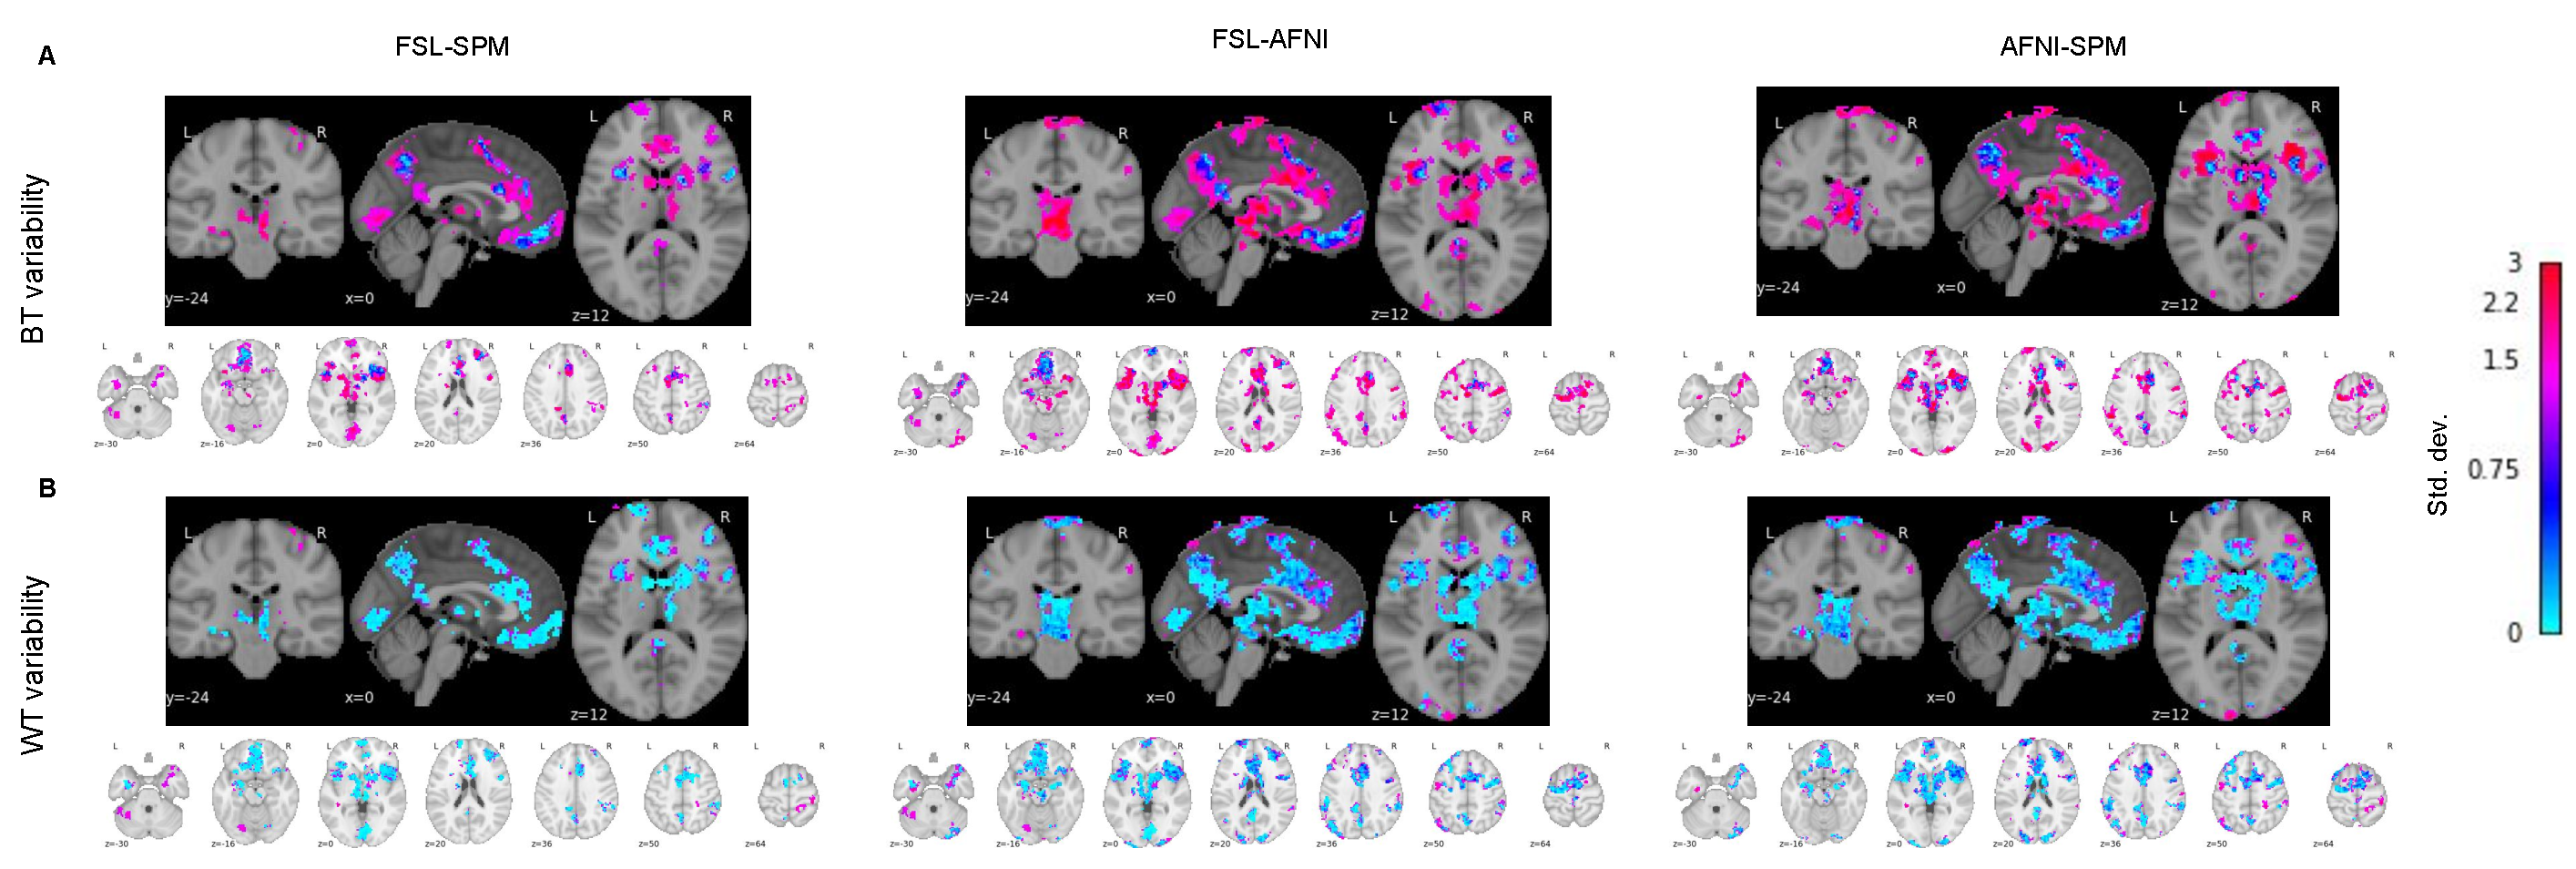
\includegraphics[width=\textwidth]{figures/bt-wt-thresh-std.pdf}
      %\caption{Standard deviation of thresholded t-statistics map on template surface}
    \end{subfigure}
    \hfill
    \begin{subfigure}[t]{\textwidth}
      \centering
      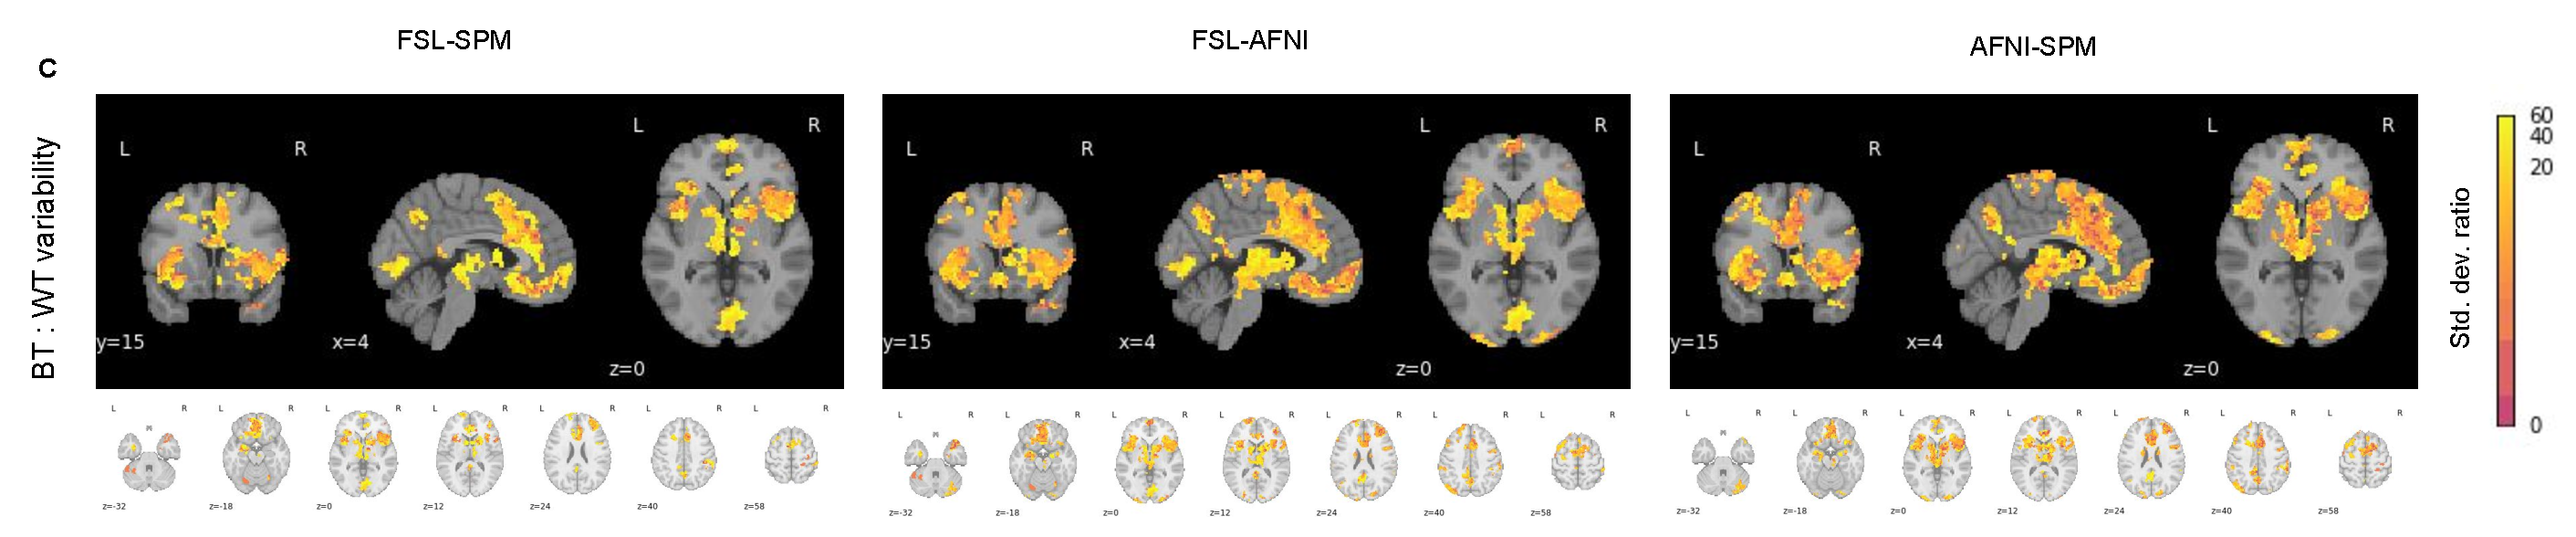
\includegraphics[width=\textwidth]{figures/ratio-thresh-std.pdf}
      %\caption{Standard deviation of thresholded t-statistics map on template surface}
    \end{subfigure}
    \caption{Maps of standard deviation of thresholded T-statistics. The first and second rows show
    maps on BT and WT results, respectively, and the third row represents maps of the ratio between them.}
    % so that bright blue areas indicate more similar order of magnitude of variations in both conditions,
    %and vise versa for the darkder regions.}
    \label{fig:thresh-maps}
    \end{minipage}}
  \end{figure*}


  %%%%%%%%%% Dice plot of thresholded tstats%%%%%%%%
  \begin{figure}[b]
    \fbox{\begin{minipage}{\dimexpr \columnwidth-2\fboxsep-2\fboxrule}
    \centering
    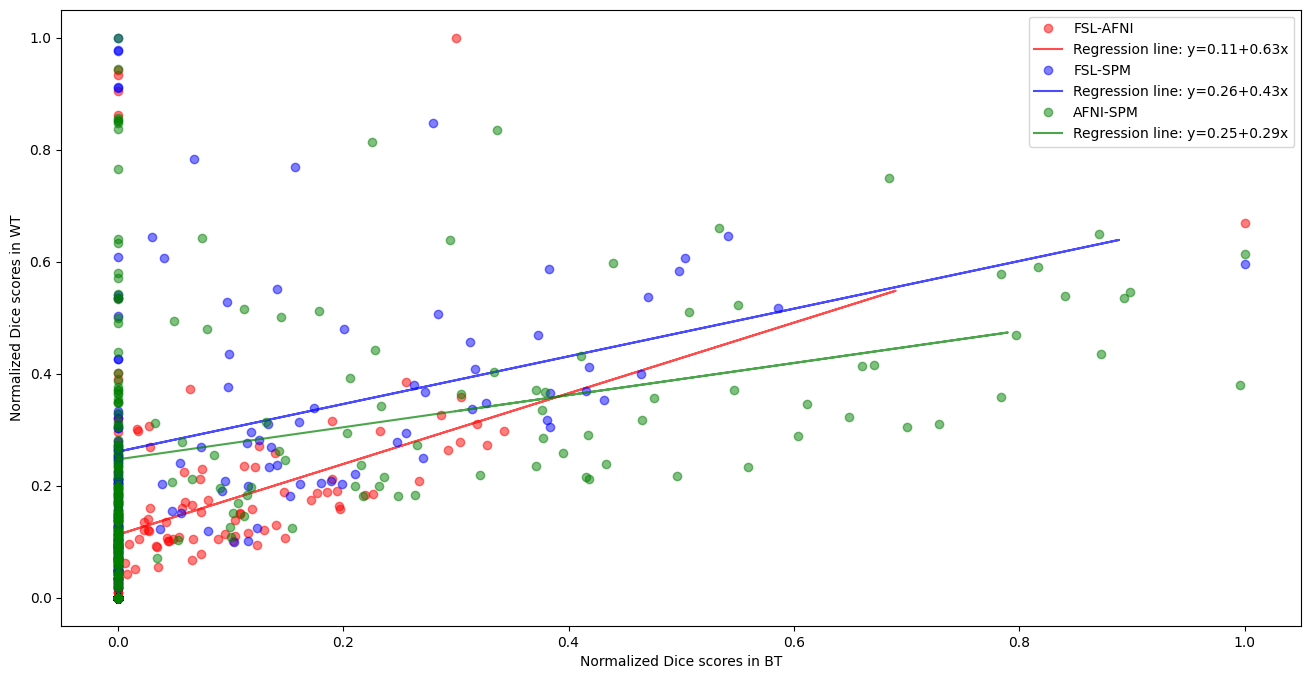
\includegraphics[width=\columnwidth]{figures/dices_corr.png}
    \caption{Correlation of Dice coefficients of activated regions in BT and WT
    from the thresholded T-statistics. Different pairs are illustrated in different colors.
    Regions correspond to the 360 areas of cortical parcellation (HCP-MMP1.0)~\cite{glasser2016multi}.}
    \label{fig:dice-thresh}
    \end{minipage}}
  \end{figure}



\subsection{Group-level unthresholded maps}
% \subsection{Variability of unthresholded statistical maps}

% Fig3
Figure~\ref{fig:unthresh-maps} shows the brain maps of standard deviations for group-level unthresholded T-statistics in WT and BT.
Results show a different magnitude of
the order of variations in WT and BT with standard deviation ranges from $\approx$ 0.12 to $\approx$ 0.5 on average, respectively.
The maps show regions in the brain where the magnitude of standard deviation is close to zero in WT but it exceeds 2.0 in BT,
such as the limbic and frontal lobes in the sagittal plane.
However, there are voxels with a significant correlation between WT and BT that are uniformly distributed across the brain maps.

%%%%%%%%%% Var. of Unthresh %%%%%%%%
\begin{figure*}[b]
    \fbox{\begin{minipage}{\dimexpr \textwidth-2\fboxsep-2\fboxrule}
    \begin{subfigure}[t]{\textwidth}
      \centering
      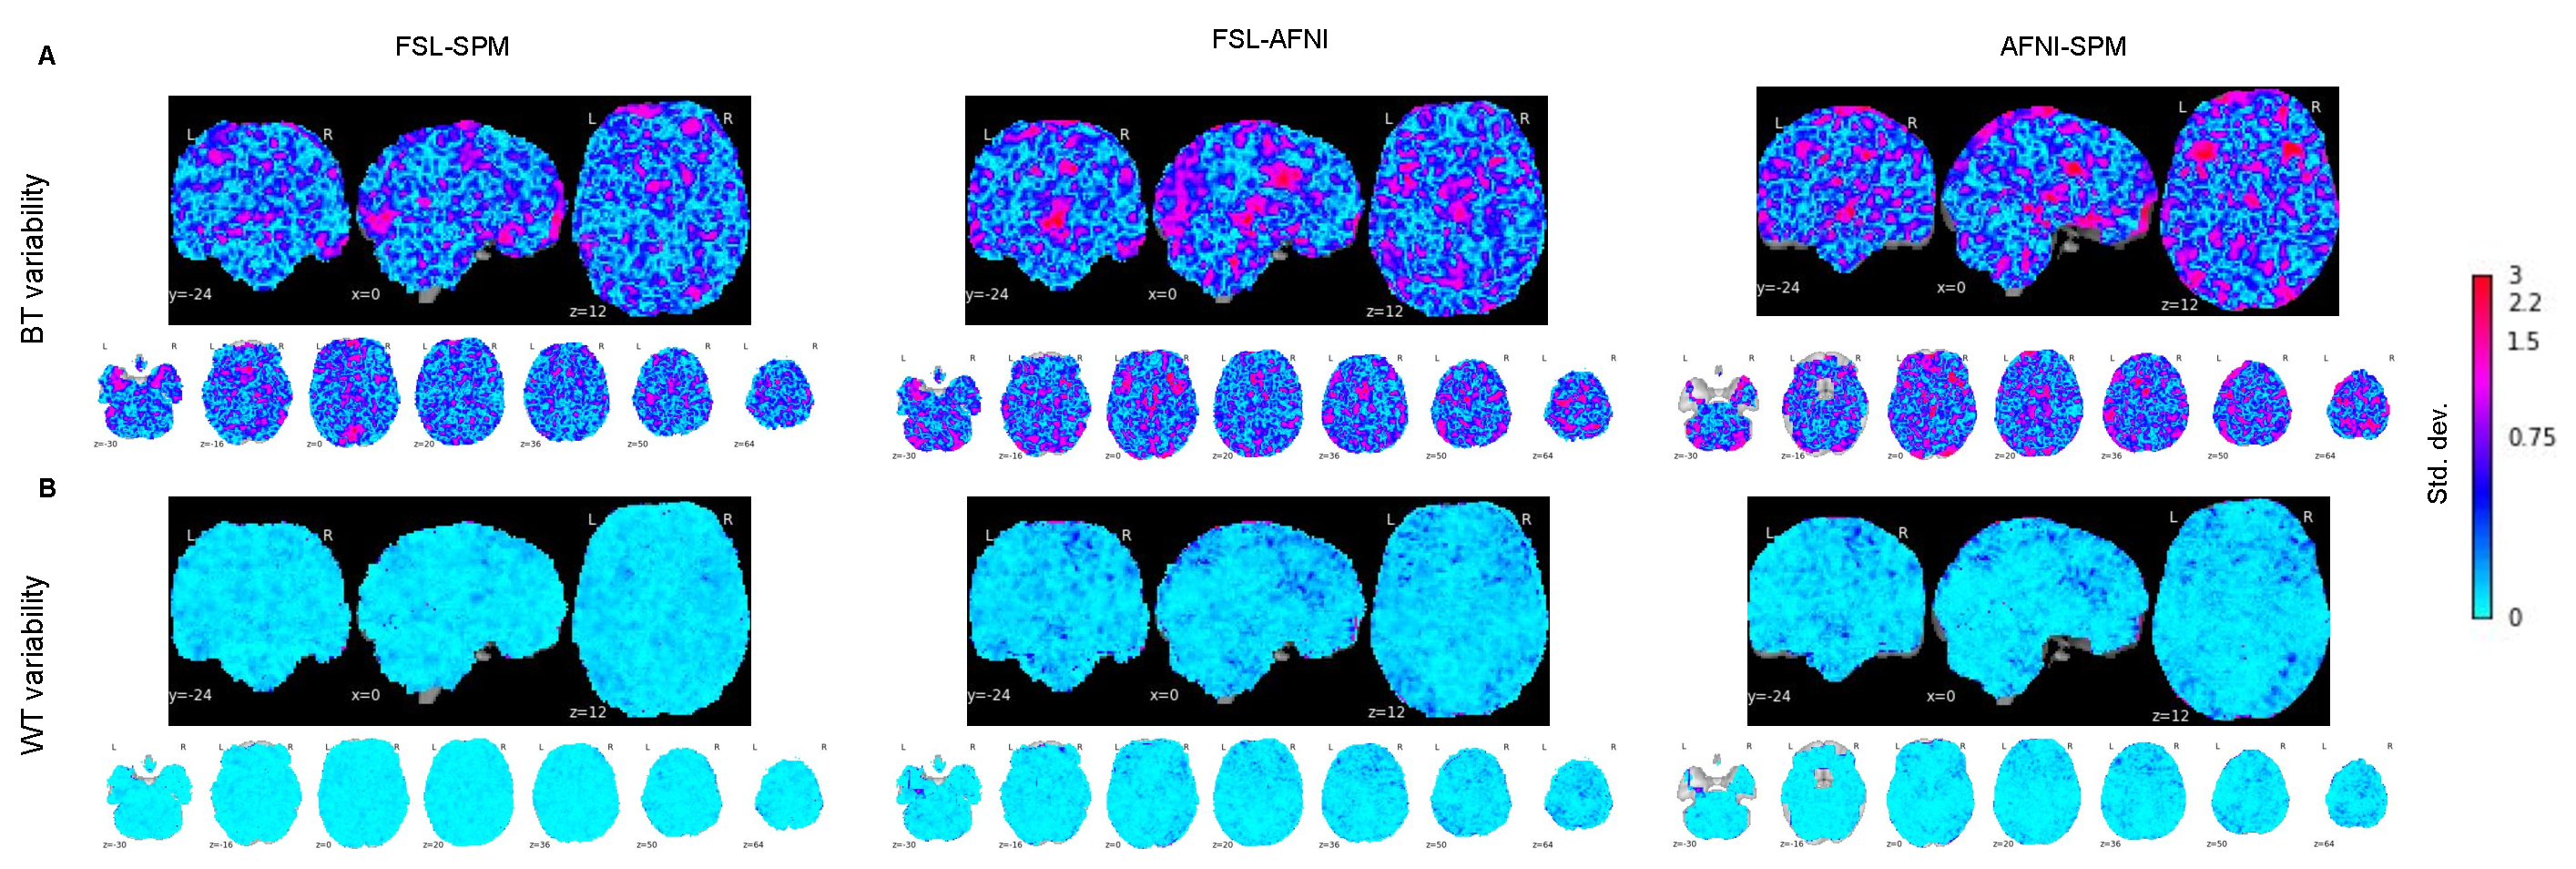
\includegraphics[width=\textwidth]{figures/bt-wt-unthresh-std.pdf}
      %\caption{Standard deviation of thresholded t-statistics map on template surface}
    \end{subfigure}
    \hfill
    \begin{subfigure}[t]{\textwidth}
      \centering
      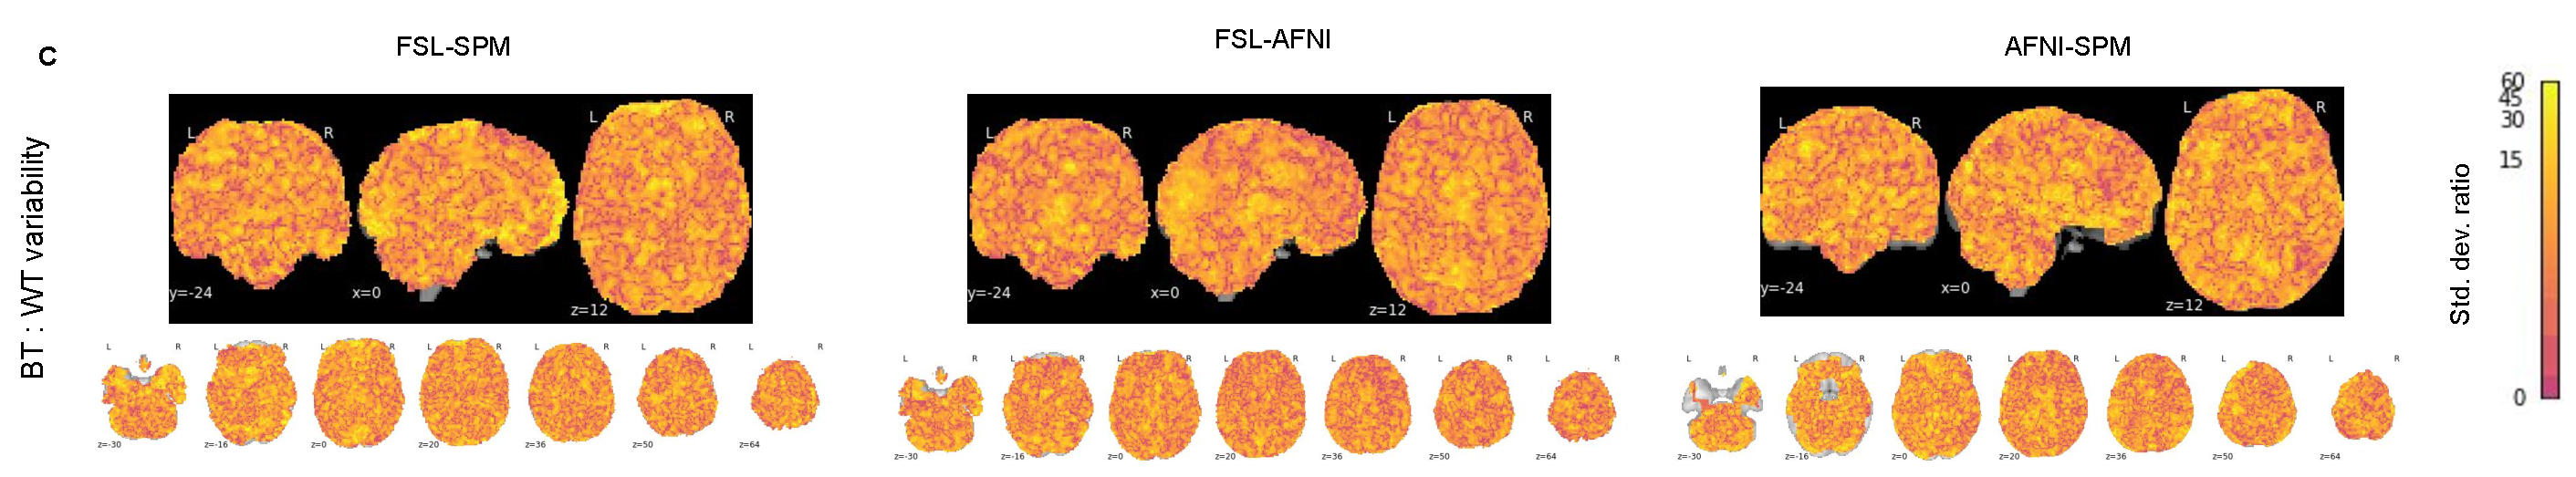
\includegraphics[width=\textwidth]{figures/ratio-unthresh-std.pdf}
      %\caption{Standard deviation of thresholded t-statistics map on template surface}
    \end{subfigure}
    \caption{Maps of standard deviation of unthresholded T-statistics. The first and second rows show
    maps on BT and WT results, respectively, and the third row represents maps of the ratio between them.}
    \label{fig:unthresh-maps}
    \end{minipage}}
  \end{figure*}


% Fig4
The scatter plot in Figure~\ref{fig:unthresh-correlation} represents the correlation of standard deviation in WT and BT variability.
We found two major clusters, including the identity cluster that corresponds to the correlations
between BT and WT with the ratio of $0.5 < BT/WT < 2$ where the standard deviations are bigger than 0.1,
and the upper cluster that shows voxels where BT $\approx$ 0.
The percentage of voxels included in the identity cluster is \%9.9 in \fslspm, \%17.3 in \fslafni, and \%13.8 in \afnispm,
and in the upper cluster is $\approx$ \%1 for each pair of tools.
The identity area is also represented on the MNI space in the second row in Figure~\ref{fig:unthresh-correlation}.
This figure shows the spatial localization of the parts of the brain that BT variability is correlated with the numerical variability.
This refines the presented results in Figure~\ref{fig:unthresh-maps},
which indicates how correlation is uniformly distributed across the brain.

  %%%%%%%%%% Corr. plot of tstats%%%%%%%%
  \begin{figure*}[b]
    \fbox{\begin{minipage}{\dimexpr \textwidth-2\fboxsep-2\fboxrule}
      \begin{subfigure}[t]{\textwidth}
        \centering
        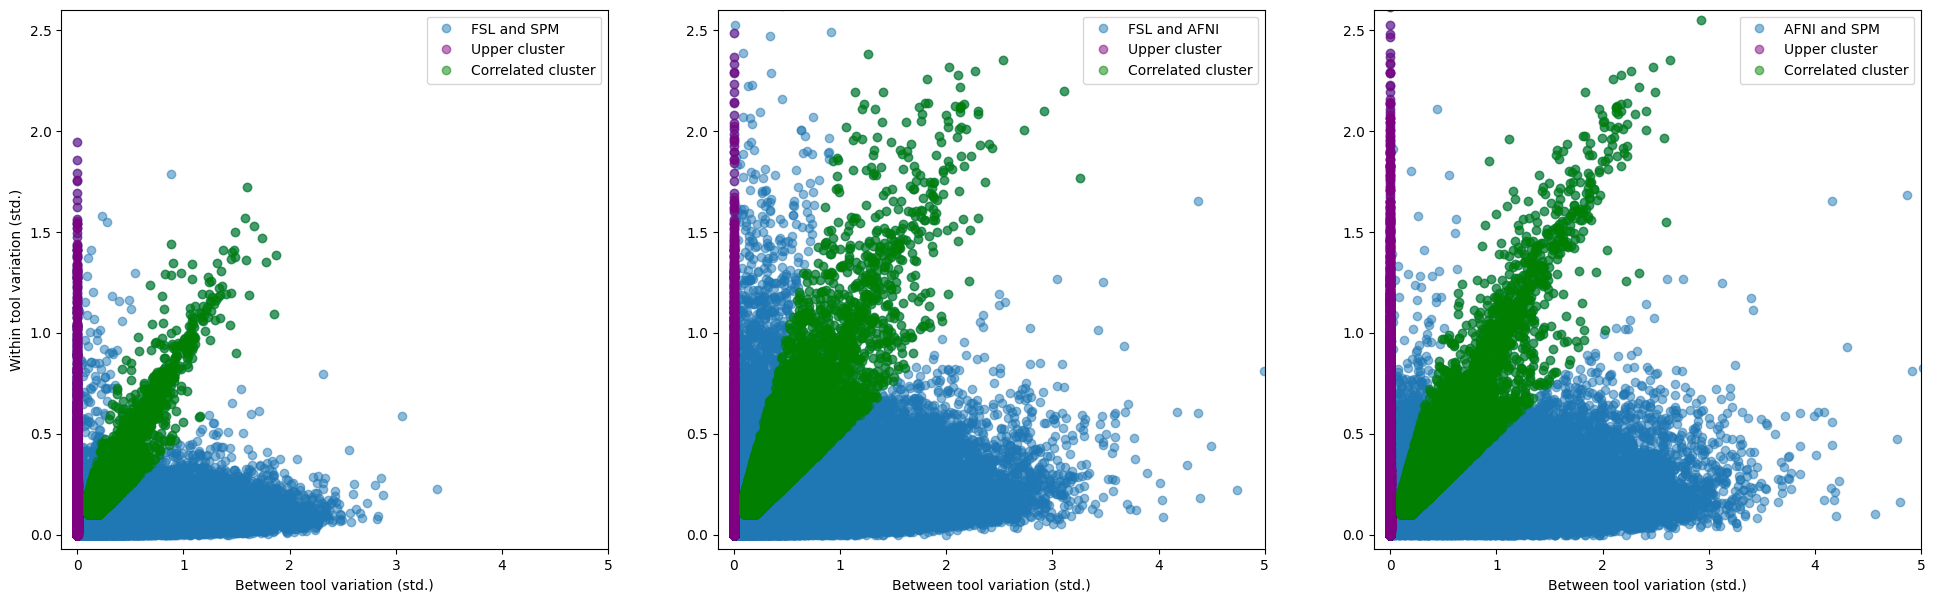
\includegraphics[width=\textwidth]{figures/std-corr-unthresh-plot.png}
        %\caption{Standard deviation of thresholded t-statistics map on template surface}
      \end{subfigure}
      \hfill
      \begin{subfigure}[t]{\textwidth}
        \centering
        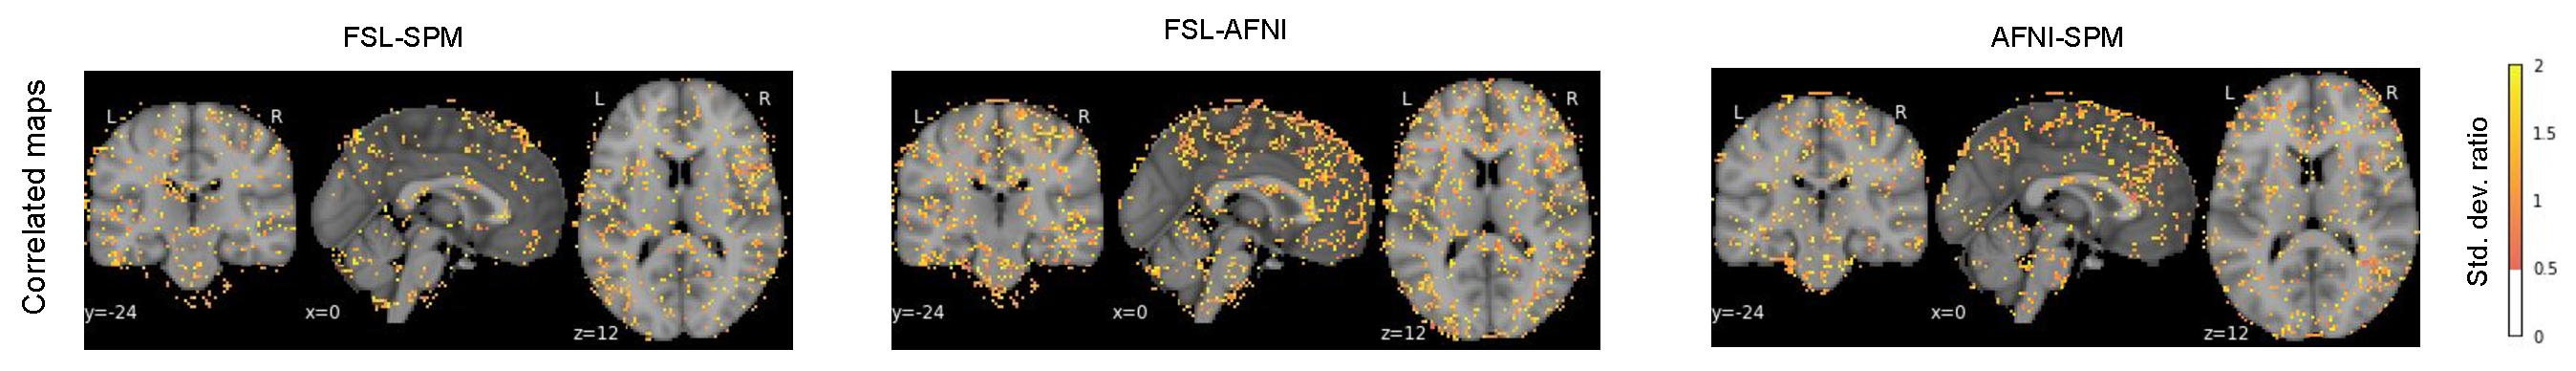
\includegraphics[width=\textwidth]{figures/corr-unthresh-std.pdf}
        %\caption{Standard deviation of thresholded t-statistics map on template surface}
      \end{subfigure}
      \caption{Correlation of standard deviations in BT and WT from the unthresholded T-statistics.
      The first row plots the correlations voxel by voxel and is highlighted with different colors
      for two clusters, including the upper cluster (purple color) and the correlated cluster (green color).
      The second row maps the correlated area on the MNI space.}
    \label{fig:unthresh-correlation}
    \end{minipage}}
  \end{figure*}


  \subsection{Subject-level unthresholded maps}

  Table~\ref{table:firstlevel-stats} shows a summary of the statistics from the subject-level analysis results.
  This table represents the average of the mean and standard deviation of absolute differences of unthresholded T-statistics
  across 16 subjects for each pair of tools.
  Results show the subjects that were produced the least and the most variability among all pairs, subjects,
  and both BT and WT.
  While the subject with the least variability generated results with the mean of $\approx$ 0.093 and standard deviation of $\approx$ 0.174,
  the subject with the most variability produced results with the mean of $\approx$ 0.183 and standard deviation of $\approx$ 0.341.
  This observation shows an order of magnitude of variability between subjects.
  % The most variability for \fslspm appeared in subject 1 in BT and subject 11 in WT, and for \fslafni
  % and \afnispm subject 10 in BT and subject 5 in WT were the most variable subjects.
  % Moreover, Figure~\ref{fig:unthresh-firstlevel} shows the maps of standard deviations on MNI space in WT and BT for subjects 15 and 10.
  % We can see a significant variability between subjects.

  Moreover, Figure~\ref{fig:unthresh-maps-sbj} shows the maps of standard deviations on MNI space in WT and BT from T-statistics of
  the subject with the highest WT variability.
  The average standard deviations in WT and BT are $\approx$ 0.152 and $\approx$ 0.466, respectively.
  The maps show regions in the brain where the magnitude of standard deviation exceeds 1.0 in WT in \fslafni and \afnispm,
  such as the parts in the frontal and occipital lobes.



%%%%%%%%%% Summary of statstics %%%%%%%%
\setlength{\tabcolsep}{5pt}
\begin{table*}[h]
    \centering
    \begin{tabular}{cccc|cc|cc}
        \toprule
        \multirow{2}{*}{} &{} & \multicolumn{2}{c}{All Subjects} & \multicolumn{2}{c}{Least variable} & \multicolumn{2}{c}{Most variable} \\
        \cmidrule{3-4} \cmidrule{5-6} \cmidrule{7-8} \\
        {} & {} & Mean  & Std. dev.  & Mean & Std. dev. & Mean  & Std. dev. \\
        \midrule
        \rowcolor{lightgray}
        {BT} & FSL vs. SPM           & 0.245     & 0.366       & 0.166     & 0.255    & 0.273    & 0.405  \\
        \rowcolor{lightgray}
        {}   & FSL vs. AFNI          & 0.295     & 0.439      & 0.183     & 0.282     & 0.392    & 0.582  \\
        \rowcolor{lightgray}
        {}   & AFNI vs. SPM          & 0.238     & 0.491      & 0.150     & 0.314     & 0.310    & 0.642  \\
        {WT} & FSL and SPM    & 0.033     & 0.092      & 0.018     & 0.050     & 0.036    & 0.099  \\
        {}   & FSL and AFNI   & 0.040     & 0.136      & 0.021     & 0.075     & 0.048    & 0.165  \\
        {}   & AFNI and SPM   & 0.033     & 0.124      & 0.019     & 0.071     & 0.039    & 0.155  \\
        \bottomrule
    \end{tabular}
    \caption{Summary of voxel-wise mean and standard deviation of absolute differences for each pair of tools
    in subject-level T-statistics.}
    \label{table:firstlevel-stats}
\end{table*}


  % %%%%%%%%%% Var. of Unthresh %%%%%%%%
  % \begin{figure*}[b]
  %   \fbox{\begin{minipage}{\dimexpr \textwidth-2\fboxsep-2\fboxrule}
  %     \centering
  %     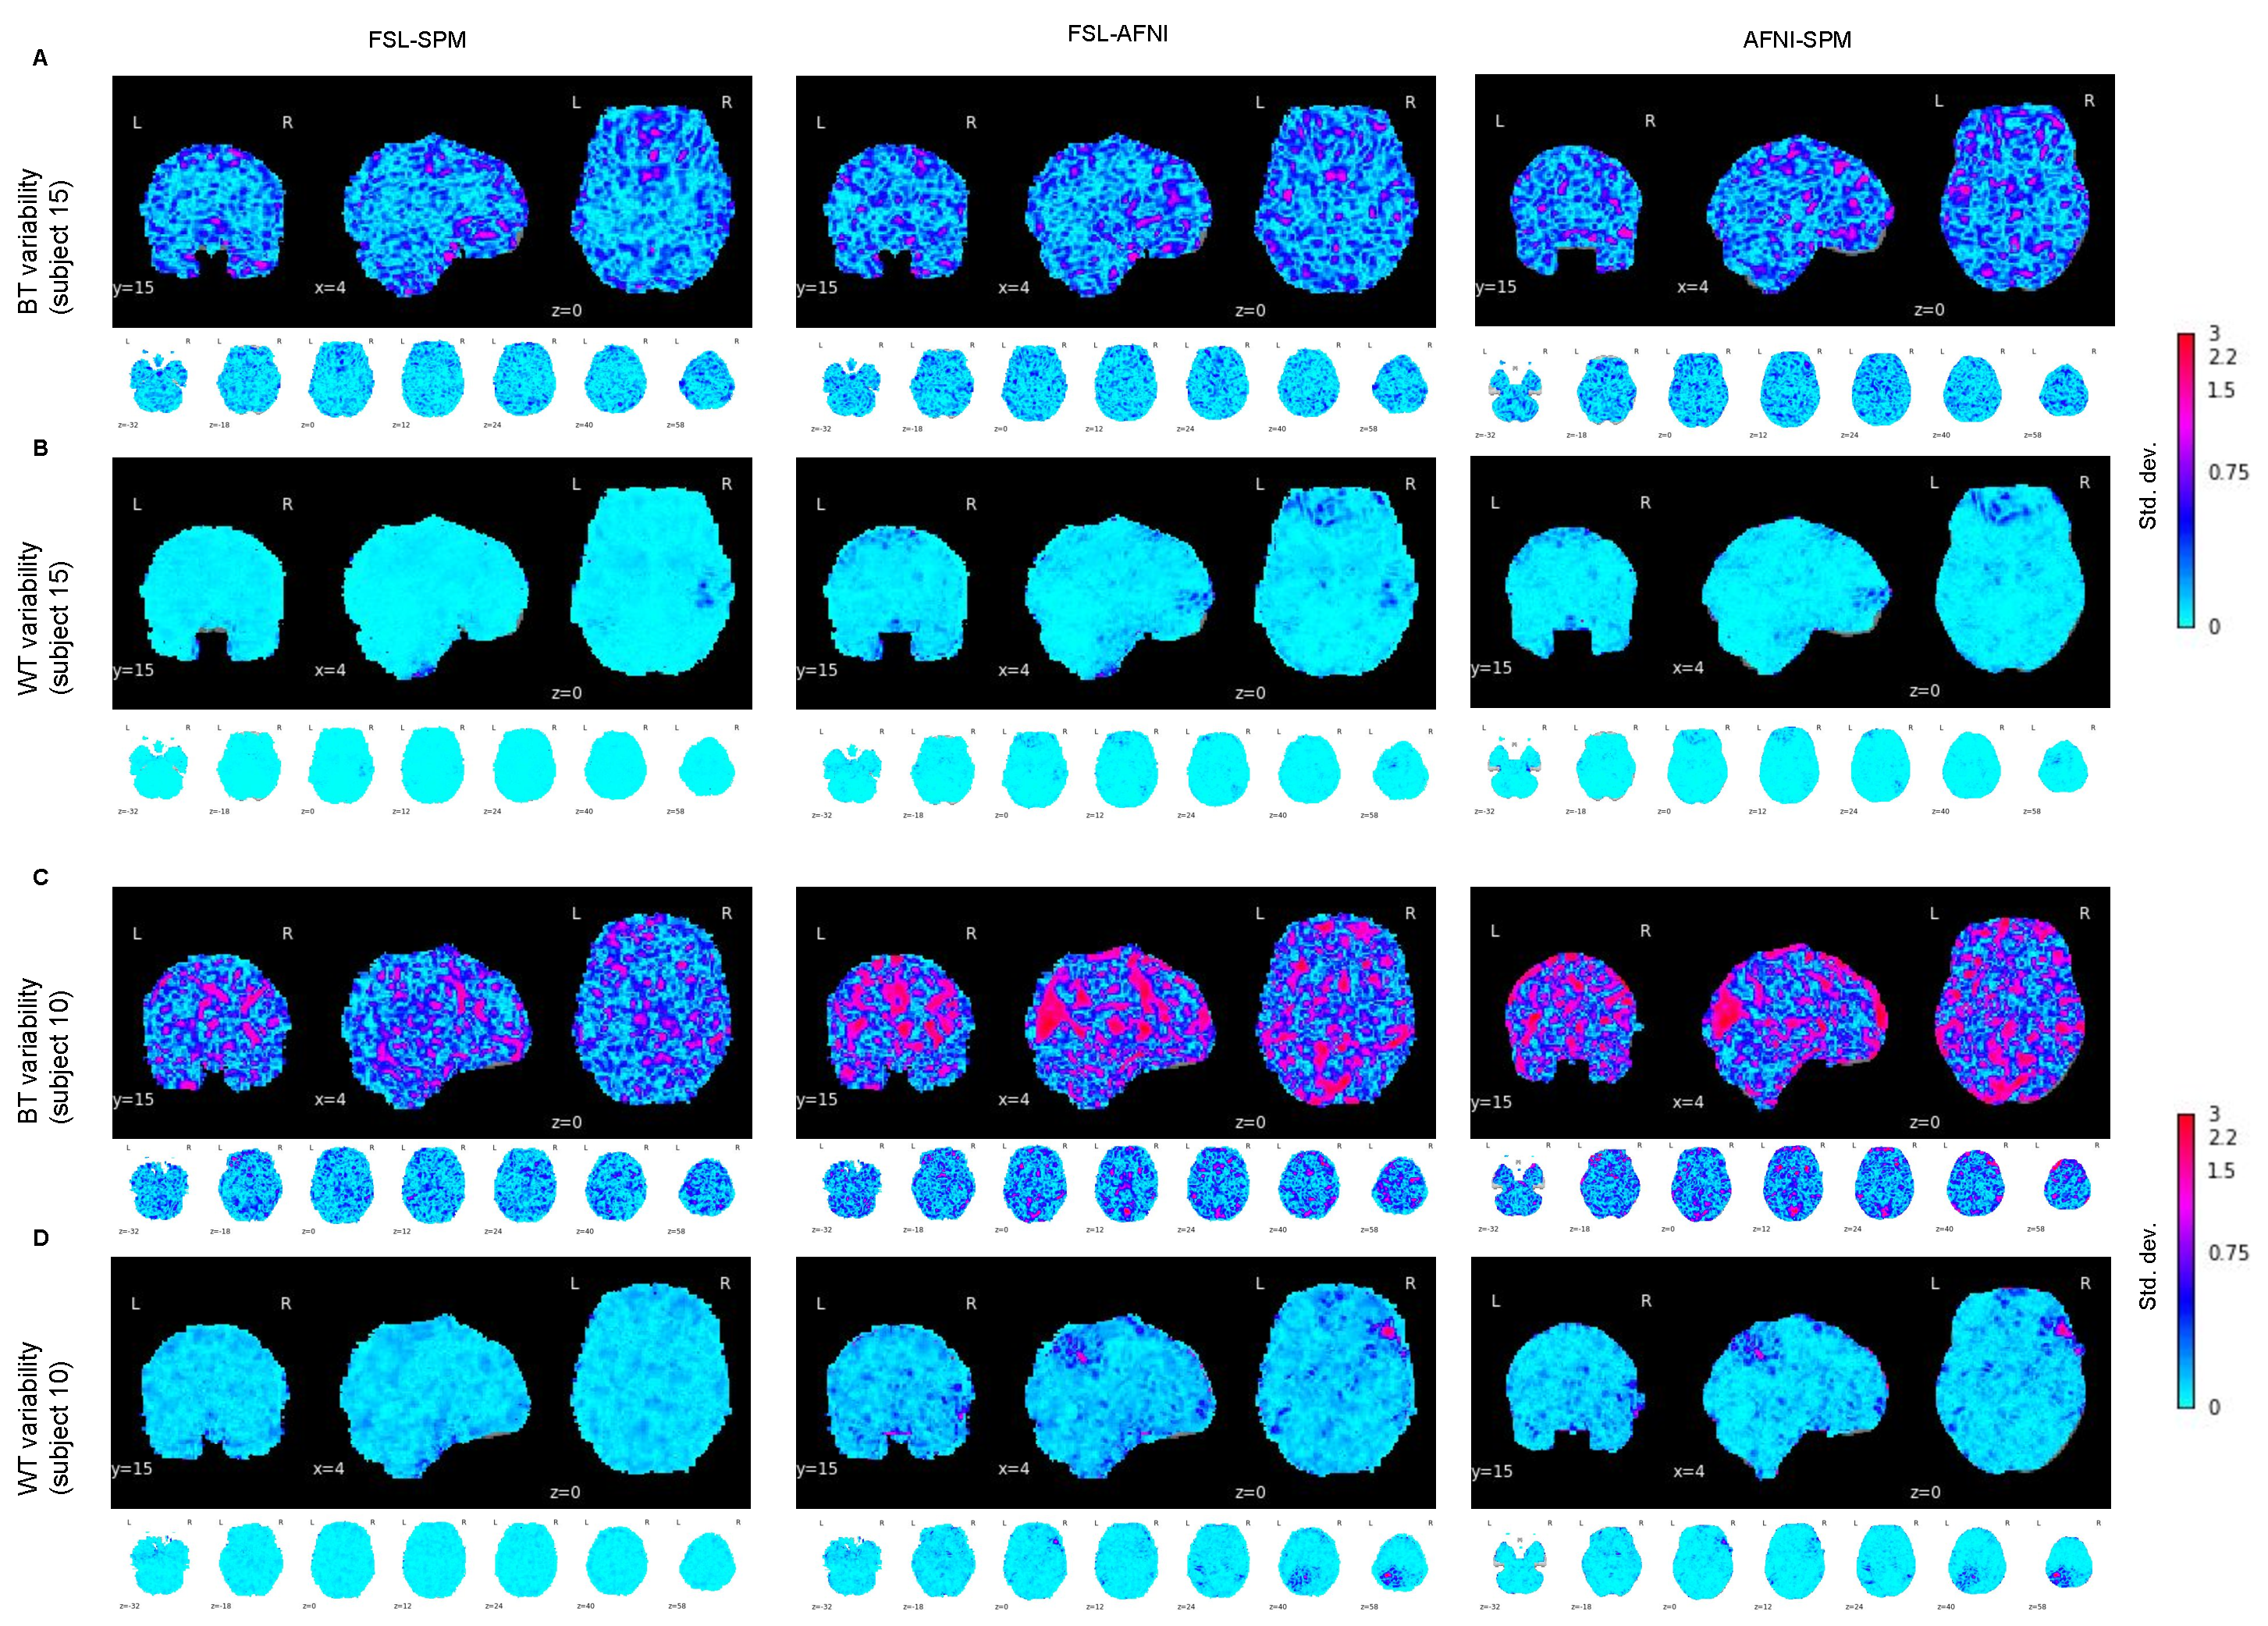
\includegraphics[width=\textwidth]{figures/sbj-level-bt-wt-unthresh-std.pdf}
  %   \caption{Maps of standard deviation of unthresholded T-statistics from subject 15 in the rows A and B,
  %   and subject 10 in the rows C and D.}
  %   \label{fig:unthresh-firstlevel}
  %   \end{minipage}}
  % \end{figure*}


  %%%%%%%%%% Var. of Unthresh sbj05%%%%%%%%
\begin{figure*}[b]
  \fbox{\begin{minipage}{\dimexpr \textwidth-2\fboxsep-2\fboxrule}
  \begin{subfigure}[t]{\textwidth}
    \centering
    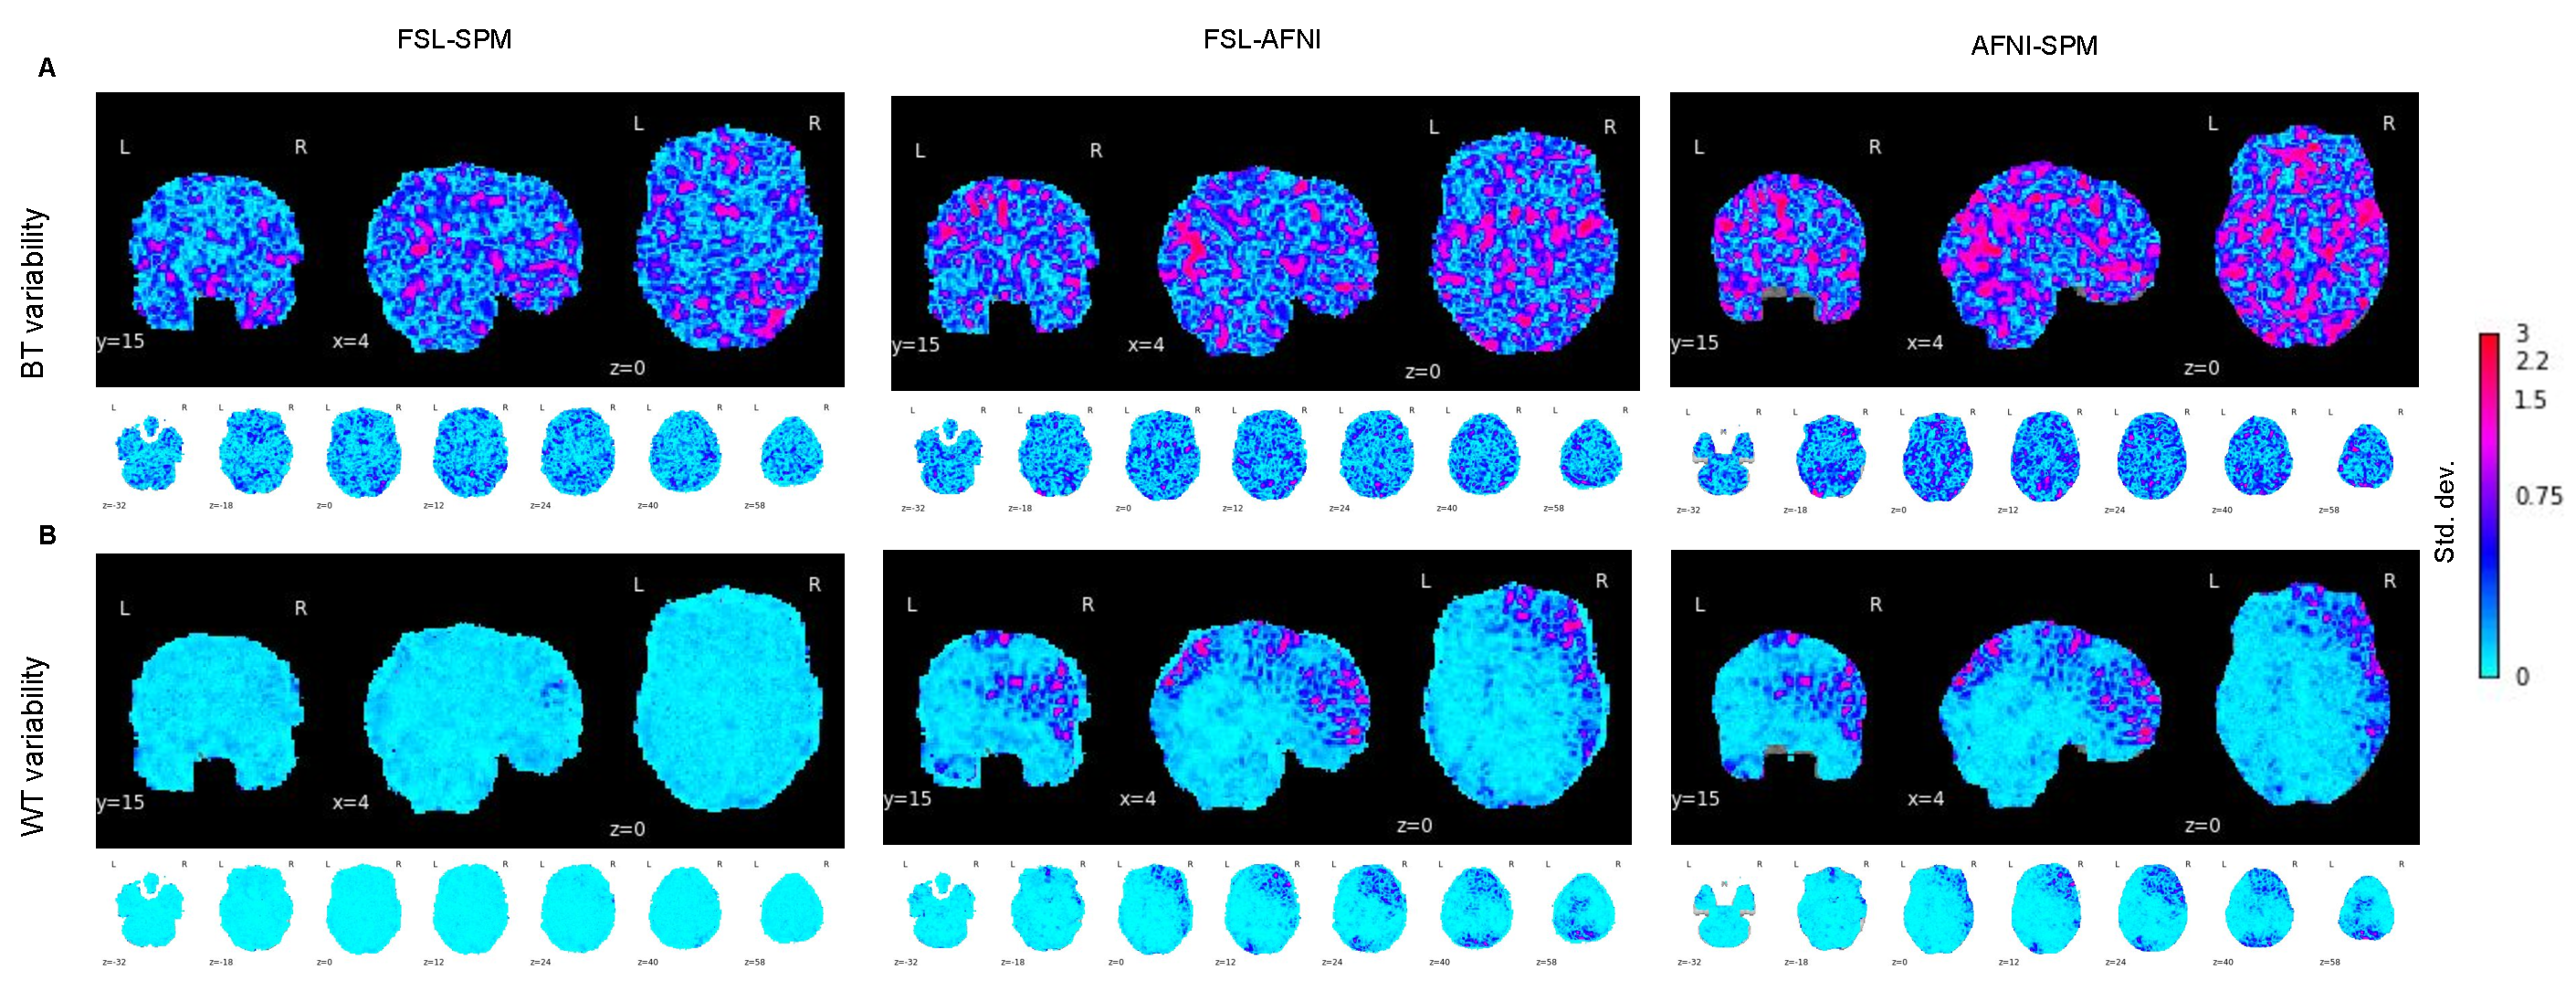
\includegraphics[width=\textwidth]{figures/sbj05-bt-wt-unthresh-std.pdf}
    %\caption{Standard deviation of thresholded t-statistics map on template surface}
  \end{subfigure}
  \hfill
  \begin{subfigure}[t]{\textwidth}
    \centering
    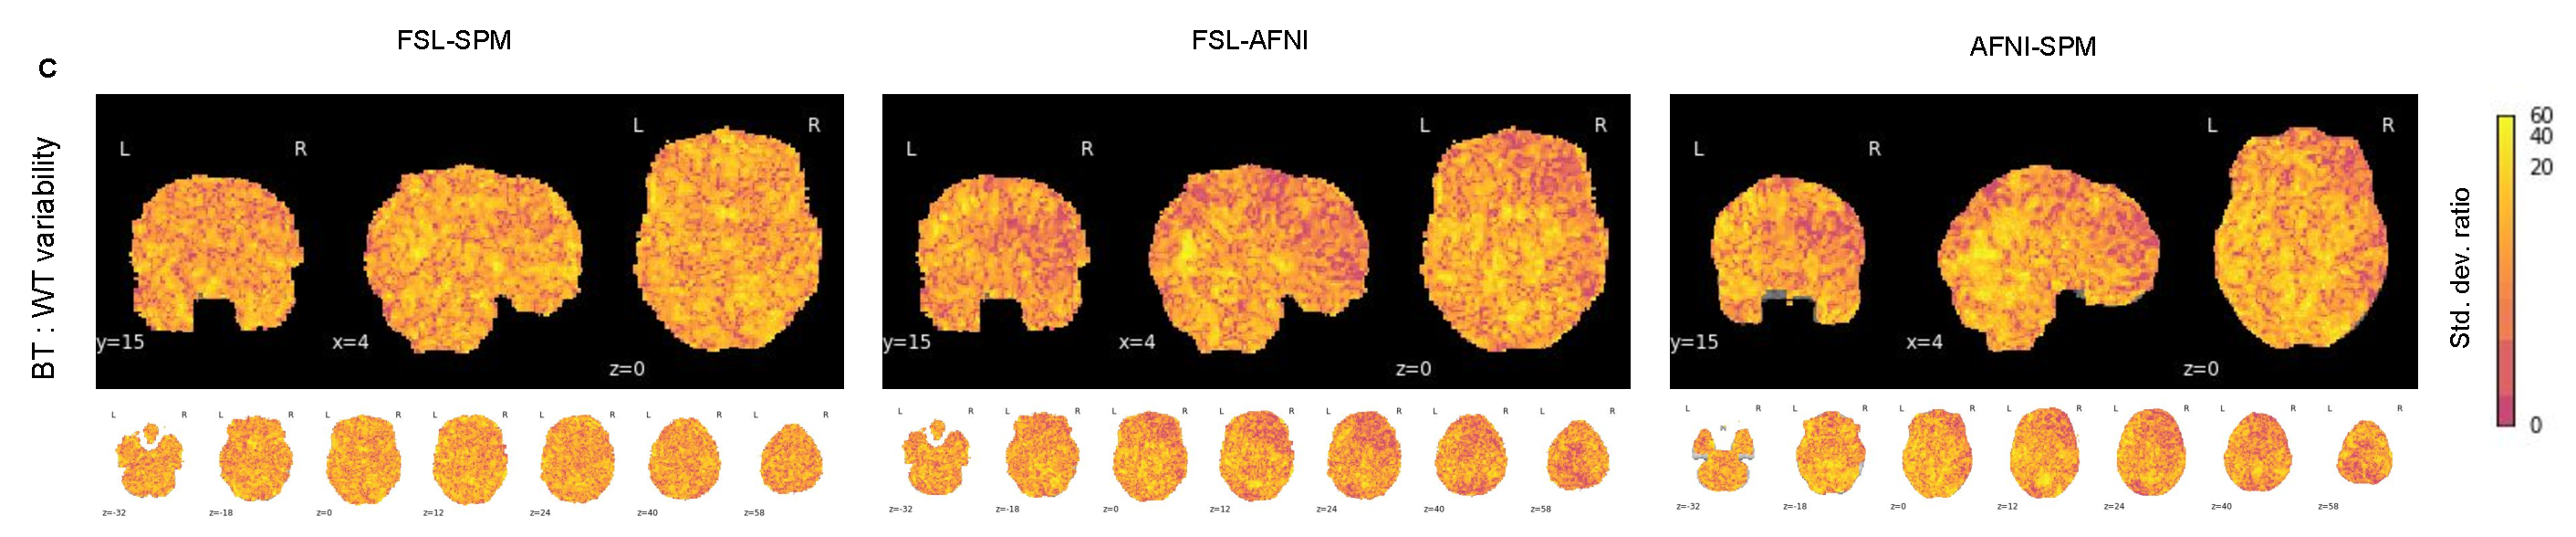
\includegraphics[width=\textwidth]{figures/sbj05-ratio-unthresh-std.pdf}
    %\caption{Standard deviation of thresholded t-statistics map on template surface}
  \end{subfigure}
  \caption{Maps of standard deviation of unthresholded T-statistics in subject 5. The first and second rows show
  maps on BT and WT results, respectively, and the third row represents maps of the ratio between them.}
  \label{fig:unthresh-maps-sbj}
  \end{minipage}}
\end{figure*}


\section{Conclusion \& Discussion}

% There are many statistical comparisons, but the neuro-scientific interpretation of results is not on my side.

\begin{itemize}
    \item[$\bullet$ ] In this study, we represented the magnitude of differences in between tool and within tool results.
    We obtained more instability in BT compared to WT. Also we showed how between tool variations
    are correlated with numerical variability.

    \item[$\bullet$ ] Generally, we obtained more uncertainty on thresholded results, probably due to different thresholding
    methods used in different tools. This can raise further investigations on the thresholding techniques toward stability.

    \item[$\bullet$ ] Further studies can be evaluating the numerical stabilities within tool by focusing on the particular parts of
    the pipeline that has been identified as the main sources of variations in~\cite{bowring2021isolating}.
    Also, we can invetigate the precision in WT variability that simulates mostly BT variability in the furure study.

\end{itemize}


\section{Acknowledgments}


%%
%% The next two lines define the bibliography style to be used, and
%% the bibliography file.
\bibliographystyle{plain}
\bibliography{biblio}


\end{document}
\endinput
%%
%% End of file `sample-authordraft.tex'.
